\documentclass{subfiles}

\begin{document}

In this section, we explain the details of the Acquire data in practical terms. Even though the entire thesis is focused on

 in terms of scientific background as well as practical output. 

There are two types of LiDAR data, the discrete and the FW. The discrete LiDAR records a few peak laser returns, while the FW LiDAR records the entire backscattered signal \cite{Wanger2004}. This suggests new possibilities but also many new problems from the point of view of data processing and visualisation. Nevertheless, FW LiDAR data has a better vertical profile and as shown at \cite{Anderson2015} and worth the extra processing required in comparison to discrete LiDAR.
\par The primary output of this research is the open source software DASOS (=forest in Greek), which aims to enhance visualisation and classifications of FW LiDAR. In this extended abstract, we sum up previous visualisation research applied using DASOS \cite{Miltiadou2014} \cite{Miltiadou2015}, as well as the future directions of FW LiDAR visualisations. This work is divided into three sub-section:

The data that we are using are shown in the figure below:

Data
LiDAR \& hyperspectral
discrete full-waveform
for Instruments 


\begin{figure}
	\centering
	\includegraphics[width=\textwidth]{img/Data_n_Instruments}
	\caption{Data and Instruments}
\end{figure}

\begin{figure}
	\centering
	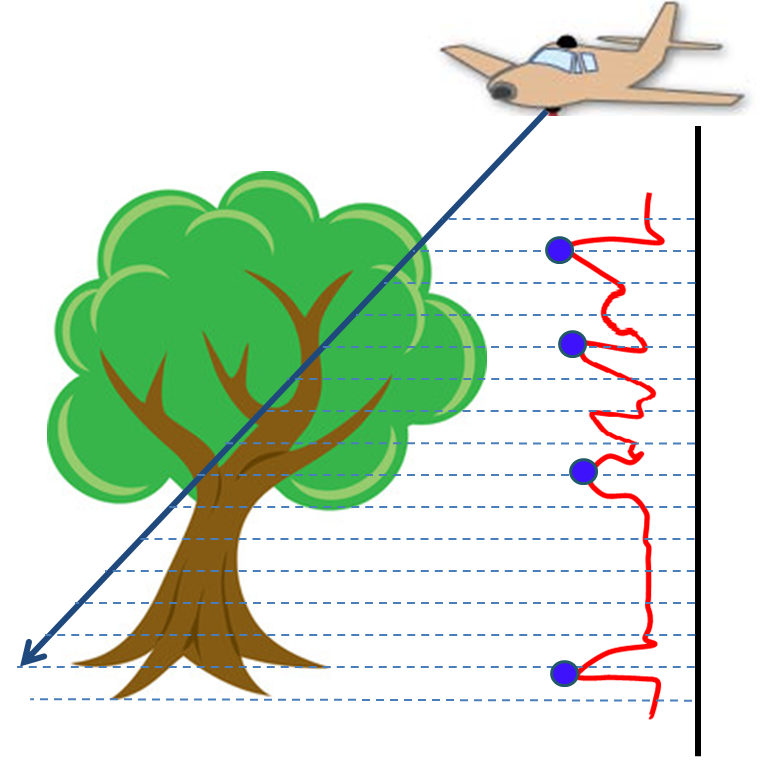
\includegraphics[width=\textwidth/3*2]{img/LiDAR_DiscretVsFW_fig}
	\caption{Discrete and FW LiDAR data System}
\end{figure}


two organisation:
	1. Natural Environment Research Council’s Airborne Research and Survey Facility (NERC ARSF)
	2. Interpine Ltd Group () 
	
	1. used for the hyperspectral Alignment
	2. dead tree detection
	both for visualisations and optimisations of various data structures
	
	\section{Instrumenets}
	1. Instruments 
		- Leica ALS50-II
		- AISA Eagle and Hawk
		
	2. Instrument
		- Riegl LMS-Q680i
	
	\par 
	, which aims to break the barrier between understanding and using the FW LiDAR.
	

	The sample data used for this thesis are provided by Natural Environment Research Council’s Airborne Research and Survey Facility (NERC ARSF). The datasets mainly used were scanned on the 8th of April in 2010 at New Forest in UK. For every flightline, two Airborne Remote Sensing datasets are given: 
	
	-	Full-waveform (FW) LiDAR data collected from the Leica ALS50-II system
	-	Hyperspectral Images collected from the AISA Eagle and Hawk instruments
	
	For each flightline, there is a FW LiDAR file, as well as the corresponding hyperspectral data. But since the data are collected from different instruments they are not aligned (see section 5 for more information on aligning the data). 
	
	In the following sub-sections, background information on the input datasets is given, starting from simple concepts like Remote Sensing. Then, the inputs are explained in practise; what the actual input data are and how they are interpreted. The challenges of dealing with the data are also outlined and discussed. 


	\par Nevertheless, the newest sensors RIEGL LMS-Q780 and RIEGL LMS-Q680i are native full-waveform sensors and the discrete LiDAR are produced by extracting peak points at post-processing. Therefore the concept of extracting a denser point clouds using Gaussian decomposition does not apply on data collected from those sensors. That was also proved by extracting peak points from RIEGL FW LiDAR data using the pulseextract from LAStools ~\cite{LAStools}. The number of points extracted was exactly the same as the number of points saved into the associated discrete LiDAR files.


	\section{Full-waveformLiDAR}
	


	
	\section{Hyperspectral Imagery}
	
	
\end{document}